\chapter{Joint Decisions \who{Dubernet}}
\label{ch:jointtrips}
% ##################################################################################################################

\hfill \textbf{Author:} Thibaut Dubernet

\begin{center} 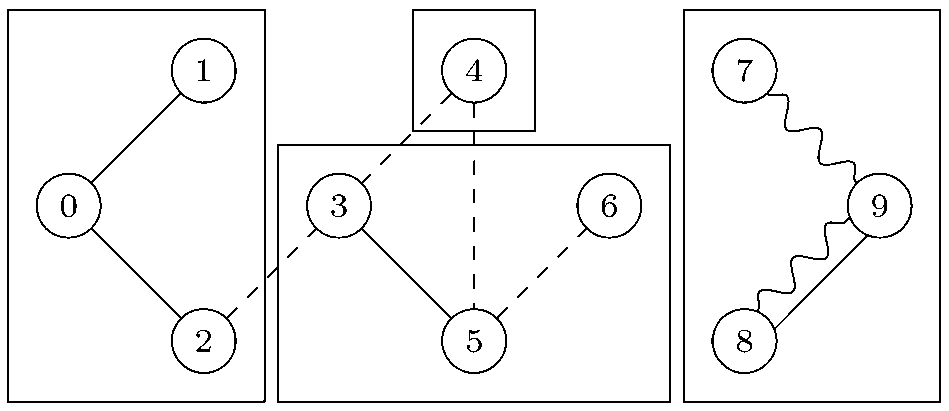
\includegraphics[width=0.4\textwidth, angle=0]{extending/figures/Jointtrips/group.png} \end{center}

% ##################################################################################################################

\newcommand\authoranddate{\citet}

\authoranddate{DubernetAxhausen_unpub_Frontiers_2013, DubernetAxhausen_unpub_SmartCities_2013, DubernetAxhausen_STRC_2014,DubernetAxhausen_Transportation_forth}

\section{Joint Decisions and Transport Systems}
%!!!!!!!!!!!!!!!!!!!!!!!!!!!!!!!!!!!!!!!!!!!!!!!!!!!!!!!!!!!!!!!!!!!!!!!!!!!!

In recent years, there has been a growing interest in the social dimension of travel,
and how travel decisions are influenced not only by the global state of the transportation system,
but also by joint decisions and interactions with social contacts.

A very active field of research is the study and modeling of intrahousehold interactions
and joint decision making, % \cite{TimmermansZhang_TransResB_2009},
often using the classical random utility framework extended to group decision making.
%
A classical way to cope with the possibly conflicting objectives of different members of the household
is to specify a group level utility function.
%
For instance,
\authoranddate{ZhangEtAl_TransResB_2005,ZhangJEtAl_TRR_2007}
develop a model where time for different activity types is allocated to household members,
subject to time constraints (including equality of time participation in joint activities),
using a group level utility function formulated as a multilinear combination of the individuals'
utilities --- that is, a linear combination of individual utilities and pair-wise
product of individual utilities;
%
% For instance,
\authoranddate{KatoMatsumoto_TransResB_2009}
use a linear combination of the utility functions of the household members as a group utility.
The assumption behind this kind of models is the existence of ``utility transfers'':
individuals accept to decrease their own utility if it allows to increase
the utility of others by a certain fraction of their loss.
%
\authoranddate{BradleyVovsha_Transportation_2005}
focus on the ``daily activity pattern'' generation,
with household ``maintenance'' tasks (\eg shopping) allocation and possibility of joint activities.
To do so, they assume a layered choice structure,
choosing first a daily activity pattern for each member,
and then assigning joint and maintenance activities.
%
\authoranddate{GliebeKoppelman_Transportation_2005} also base their model on the daily activity pattern concept,
choosing first a ``joint outcome'' (the sequence of individual and joint activities),
and then an individual pattern for each household member.
Those models rely on enumeration of the possible household level patterns.
%
\authoranddate{GliebeKoppelman_Transportation_2002}
also derived a constrained time allocation model,
which predicts the time passed by two individuals in joint activities.
Rather than postulating a group level utility function,
the models of those authors specify a special distribution for the error terms of the individuals.
In this setting,
the error term of the individuals are correlated so that the probability
of choosing a given joint output is the same for all individuals.
%
\authoranddate{HoCAndMulley_Transportation_2013} also estimate models in which members of the household
perform choices constrained by the choice of a household level travel pattern.
Their data, as well as the parameters of the models,
show high joint household activity participation on weekends,
and a high dependence of joint travel on trip purpose and household
mobility resources.
Those results highlight the importance of representing joint household decisions,
in particular when going beyond the ``typical working day''.
%
\authoranddate{VovshaGupta_Transportation_2013} formulate a time allocation model for multiple worker households,
which considers a positive utility for members of the household
to be home jointly, as it makes joint activities possible.
The estimation results show a significant influence of this kind of synchronization mechanism.
%
Most models listed in this paragraph
are specific to given household structures;
in particular, separate models need to be estimated for different household sizes.

Household level decision processes have also been modeled with approaches which significantly differ
from the classical random utility framework.
%
\authoranddate{GolobMcNally_TransResB_1997}
propose a \structeqmodel,
which predicts time allocation and trip chaining based on the sociodemographics of a household.
\authoranddate{Golob_TransResB_2000}
also used a \structeqmodel to model the dependency of time allocations
of the two heads (man and woman) of a household.
%

%
Another class of approaches,
more oriented toward multiagent simulation than analysis,
is the use of optimization algorithms to generate households plans.
They handle the household scheduling problem by transforming it into a deterministic utility maximization problem.
Contrary to the previously presented approaches,
those alternatives do not lead to the estimation of a model against data.
%However, the estimation of the utility function is usually not part of those approaches.
%
The first of those approaches was introduced by \authoranddate{Recker_TRR_1995}.
By extending increasingly the formulation of the \pudptw, a well studied combinatorial optimization problem,
he formulates the problem of optimizing the activity sequence of members of a household
as a mathematical programming problem.
%taking into account vehicle constraints, individual and household level activity,
%possibility of choosing whether to perform or not an activity, with the possibility of shared rides.
However, due to the complexity of the problem,
the full problem cannot be solved exactly by standard operations research algorithms,
and the activity durations are not part of the optimized dimensions.
\authoranddate{ChowRecker_TranResB_2012} designed an inverse optimization method
to calibrate the parameters of this model
%, including the time window constraints,
using measured data.
Also, the formulation from \authoranddate{Recker_TRR_1995}
was later extended by \authoranddate{GanRecker_TransResB_2008}
to introduce the effects of within day rescheduling due to unexpected events.
%
Another attempt to generate plans for households uses a \ga,
building on a previous \ga for individual plan generation
\cite{CharyparNagel_Transportation_2005,MeisterEtAl_Transportation_2005}.
This algorithm optimizes sequence, duration and activity choice for a household,
rewarding the fact that several members of the household perform the same activity
simultaneously, in the way also used by \authoranddate{VovshaGupta_Transportation_2013}.
%
Finally, \authoranddate{LiaoFEtAl_Transportation_2013} formulate the problem of creating
schedules for two persons traveling together as finding the shortest path
in a ``supernetwork'', and solve this problem using exact shortest path algorithms.
They however note that their model is specific to the two person problem,
and that extension to larger numbers of agents may prove to be computationally expensive.
%
%Finally, Fang \emph{et al.} optimize location and time of joint activities, constrained to time windows in pre-determined individual plans, using a multi-objective \ga \cite{Fang2011}.
All those approaches remained experimental,
and were not integrated into multiagent simulation tools.

Another class of methods aiming at multiagent simulations
is constituted rule based systems,
which use heuristic rules to construct household plans.
%
\authoranddate{MillerEtAl_Transportation_2005} develop such a model for household mode choice.
The main difference with an individual mode choice model is the consideration of household level vehicle allocation.
In their model, individuals first choose modes individually.
If a conflict occurs, the allocation that maximizes the household level utility is chosen.
The members which were not allocated a vehicle will fall back on their second best choice,
and/or examine shared rides options.
%
\authoranddate{ArentzeTimmermans_TransResB_2009}
develop a rule base model which
relies on a simulated bargaining process within the household.
Though such models can easily represent complex decision processes,
their calibration and validation is cumbersome.

Other authors have investigated the role of more general social networks on travel.
One of the main incentives to conduct such studies comes from the continuous increase of the share of
trips which are performed for leisure purpose \cite{SchlichEtAl_TransportRev_2004,Axhausen_DonaghyEtAl_2005}.
This fact represents a challenge for travel behavior modeling,
as those trips are much more difficult to forecast than commuting trips:
they are performed more sporadically, and data about those trips is much more difficult to collect
--- in particular concerning attributes of locations and events,
which are needed to make models that do not only consist of random noise.
Understanding better how destination choice for leisure trip is made is therefore essential to improve
the accuracy of those forecasts.

Various studies have been conducted with the idea that an important factor in leisure trip destination
choice, or activity duration choice, is the ability to meet social contacts.
Examples of empirical work include \authoranddate{CarrascoJAHabib_IATBR_2009}; \authoranddate{HabibCarrascoJA_TRR_2011} or \authoranddate{MooreJEtAl_Transportation_2013}.
All those studies show a substantial influence of social contacts on the spatial and temporal
distribution of activities.
%
Based on an analysis of social network involvement and role, \authoranddate{DeutschGoulias_Transportation_2013}
advocate considering the \emph{role} individuals play in different social networks.
Using latent class cluster analysis models to analyse the role of individuals in
the various social networks they are involved in,
they find that ``the decision-making role of an individual can differ vastly across different
social engagement types''.
%
\authoranddate{Frei_PhDThesis_2012} demonstrated in a simulation experiment how considering social interactions
in leisure location choice can help increase the accuracy of predicted leisure trip distance distribution.

Another field of empirical research studies the spatial characteristics of social networks.
For instance, \authoranddate{CarrascoJAEtAl_TRR_2008} studied the relationship between individual's socioeconomic
characteristics and the spatial distribution of their social contacts.
This kind of empirical work allows to specify and estimate models able to generate synthetic social networks,
given sociodemographic attributes and home location.
An example of such a model, based on the results of a survey in Switzerland,
can be found in \authoranddate{ArentzeEtAl_TRB_2012}.
This kind of model is essential if one wants to include social network interactions
in microsimulation model.

This integration of social networks in multiagent simulation frameworks has already
been attempted by other authors.
Due to their disaggregated description of the world,
such models are particularly well suited to the representation of complex social topologies.
\authoranddate{HanQEtAl_TransResPartA_2011} present experiments of using social networks
to guide activity location choice set formation in the FEATHERS multiagent simulation framework.
Using a simple scenario with 6 agents forming a \emph{clique},
%(a network where all agents have social ties with all other agents),
they consider the influence of various processes like
information exchange and adaptation to the behavior of social contacts to increase the probability
of an encounter.
They do not, however, represent \emph{joint decisions}, such as the scheduling of a joint activity.
The same kind of processes have been investigated by \authoranddate{Hackney_PhDThesis_2009},
using more complex network topologies,
within the \matsim framework, used in this paper.
\authoranddate{RonaldEtAl_TransResB_2012}
and \authoranddate{MaEtAl_TRR_2011,MaEtAl_IATBR_2012}
present agent based systems which do integrate
joint decision making mechanisms,
based on rule based simulations of a bargaining processes.
They are not yet integrated into
any operational mobility simulation platform.

% intro mon boulot
Building on all those ideas,\todo{lesquelles? preciser limitations identifies
et comment l'approche presente resoud tout}
the work presented in this paper aims at including explicit coordination of individuals
in a multiagent simulation software framework.
A game-theoretic model of joint decisions for daily planning is introduced,
and a simulation algorithm implemented using the
\matsim software framework.
The process is designed to be able to handle complex social network topologies,
%but the current implementation is restrained to a network consisting of
%isolated \emph{cliques}.
%Such a network is a good abstraction for the network of intrahousehold relationships,
%which importance should be clear from the review above.
but the current study focuses on intrahousehold ties only.
The results of an implementation for intrahousehold ridesharing
for a scenario for the Zurich area, Switzerland, are analyzed.
Comparing the results of this scenario with travel diary data,
limitations of the current implementation are identified,
and directions for future work are sketched.

\section{An Solution Algorithm for the Joint Planning Problem: a Generalization of the MATSim Process}
%!!!!!!!!!!!!!!!!!!!!!!!!!!!!!!!!!!!!!!!!!!!!!!!!!!!!!!!!!!!!!!!!!!!!!!!!!!!!

\subsection{Algorithm}
%---------------------------------------------------------------------------

\subsection{Technical Considerations on the Implementation}
%---------------------------------------------------------------------------
